\documentclass{beamer}
\usetheme{metropolis}

\usepackage{xcolor}
\usepackage{graphicx}
\usepackage{tcolorbox}
\usepackage{listings}
\usepackage{booktabs}
\usepackage{array}
\usepackage{tabularx}
\usepackage{lmodern}
\usefonttheme[onlymath]{serif}

\begin{document}
\newcommand{\tabitem}{~~\llap{\textbullet}~~}

\definecolor{codegreen}{rgb}{0,0.6,0}
\definecolor{codegray}{rgb}{0.5,0.5,0.5}
\definecolor{codepurple}{rgb}{0.58,0,0.82}
\definecolor{backcolour}{rgb}{0.95,0.95,0.92}

\lstset{
	language=C++,
	basicstyle=\scriptsize\ttfamily,
	keywordstyle=\color{magenta},
	stringstyle=\color{codepurple},
	numbers=left,
	numbersep=5pt,
	numberstyle=\tiny\color{codegray},
	backgroundcolor=\color{backcolour},
	showstringspaces=false,
	tabsize=4
}


\title{Complete Search: Introduction}
\subtitle{Try everything}
\author{UTEC - Competitive Programming}
\date{}

\maketitle

\begin{frame}
	\frametitle{Problem Solving Paradigms}

	\begin{itemize}
		\item A programming paradigm is a common pattern that can be used to solve problems.
		\item The following are the problem paradigms commonly used in competitve programming:
		\item Paradigms $=$ Algorithm?
	\end{itemize}
\end{frame}

\begin{frame}
	\frametitle{Commonly used Paradigms in Competitive Programming}
	The four problem solving paradigms commonly used in contests:
	\begin{center}
		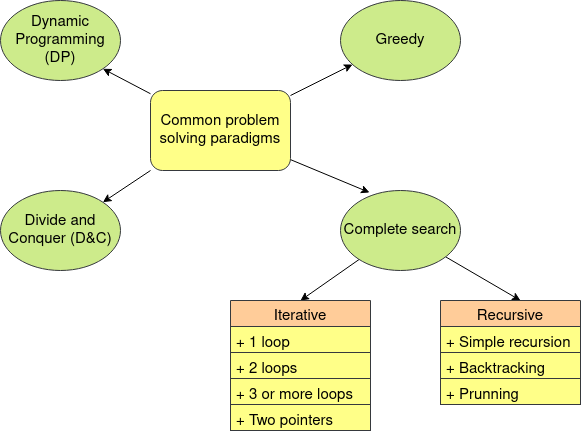
\includegraphics[scale=0.4]{images/programming-paradigms}
	\end{center}
\end{frame}

\begin{frame}
	\frametitle{Complete Search}

	\begin{itemize}
		\item Complete search is a method that can to solve almost any problem.
		\item As the name suggests, we will iterate through all possible solutions.
		\item Complete search comes in two ways: iterative and recursive.
		\item When realizing complete search in a iterative way, it is calles \textit{brute force}.
	\end{itemize}
\end{frame}

\begin{frame}
	\frametitle{Motivation}

	A pythagorean triple is a 3-tuple $(x,y,z)$ that satisfies the equation:
	$$x^2+y^2=z^2$$
	Given an integer $n$ ($n \leq 10^3$), find the number of pythagorean triples such that
	$1 \leq x, y, z \leq n$.

	\begin{itemize}
		\item Any ideas?
	\end{itemize}
\end{frame}

\begin{frame}[fragile]
	\frametitle{First Approach}
	
	We check all possible values of $x$, $y$, $z$ and see if they are a valid Pythagorean Triplet.

	\lstinputlisting{listings/first-sol.cpp}
\end{frame}

\begin{frame}[fragile]
	\frametitle{Second Approach}
	
	We can fix $x$, $y$ and check if there exists a vule of $z$ that satisfies the equation. This will improve our efficiency significantly.

	\lstinputlisting{listings/second-sol.cpp}
\end{frame}

\begin{frame}
	\frametitle{Third Approach}
	
	\begin{itemize}
		\item $x^2 + y^2 = z^2 \rightarrow (kx)^2 + (ky)^2 = (kz)^2$
		\item If $(x, y, z)$ is a Pythagorean triple and $gcd(x, y, z) = 1$, we say it is a \textit{primitive Pythagorean triple}.
		\item Thanks to Euclids Formula we know that every primitive PT can be represented as:
			$$x = a^2 - b^2$$
			$$y = 2ab$$
			$$z = a^2 + b^2$$ 
		\item So how is this useful?
	\end{itemize}
\end{frame}

\begin{frame}[fragile]
	\frametitle{Third Approach}
	Here is the implementation of the solution described above:

	\lstinputlisting{listings/third-sol.cpp}
\end{frame}

\end{document}
